\documentclass[10pt, compress]{beamer}

\usetheme{m}

\usepackage{booktabs}
\usepackage[scale=2]{ccicons}
\usepackage{minted}

\usepackage{bibentry}
\bibliographystyle{apalike}

\usepgfplotslibrary{dateplot}

\usemintedstyle{trac}

\renewcommand\footnotemark{}
\renewcommand\footnoterule{}

\title{Adding nucleo-olivary inhibition to a bottom-up computational model of the vestibulo-ocular reflex to control gaze stabilization}
\subtitle{}
\date{\today}
\author{Xavier Duran, supervised by Ivan Herreros and Paul Verschure}
\institute{Master in Cognitive Systems and Interactive Media}

\begin{document}

\maketitle


\begin{frame}[fragile]
  \frametitle{Trade-offs in avoidance actions}
  \centerline{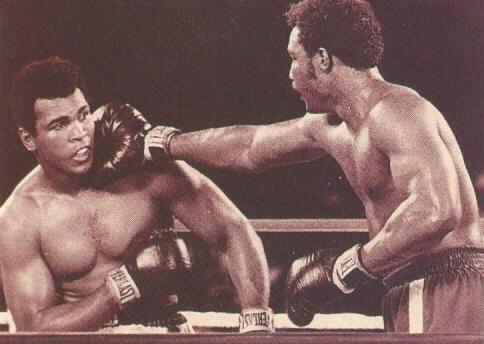
\includegraphics[scale=0.6]{images/ali.png}}
  %\footnote{\url{http://bit.ly/1OyIoEI}}
\end{frame}


\begin{frame}[fragile]
  \frametitle{Optimization of aversive reflexes}
  \begin{itemize}
    \item Avoid aversive stimuli with minimum necessary effort
    \item How we behave carries a cost: What we fail to prevent + preventing action itself
    \item The ideal actions are those that minimize the overall cost
  \end{itemize}
  \cite{Brandi2013}
\end{frame}


\begin{frame}[fragile]
  \frametitle{Cost-optimization on eye-blink reflex}
  \begin{columns}[T]
    \begin{column}[T]{5cm}
      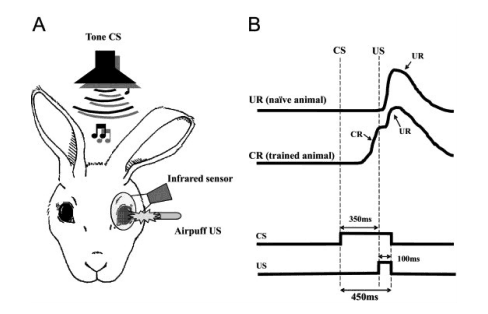
\includegraphics[scale=0.3]{images/eyeblink.png}
    \end{column}
    \begin{column}[T]{5cm}
      \begin{itemize}
        \item Perceiving an air-puff in the unprotected cornea has a cost
        \item Two types of costs
        \begin{itemize}
          \item Failing to avoid: error-based learning
          \item Avoiding when not necessary
        \end{itemize}
        \item Extinction of unnecessary conditioned responses
      \end{itemize}
      \cite{Herreros2013b}
    \end{column}
  \end{columns}
\end{frame}


\begin{frame}[fragile]
  \frametitle{Nucleo-olivary inhibition (NOI)}
  \begin{columns}[T]
    \begin{column}[T]{5cm}
      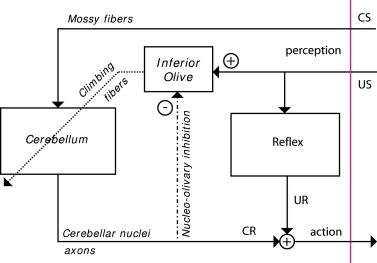
\includegraphics[scale=0.6]{images/noi.jpg}
    \end{column}
    \begin{column}[T]{5cm}
      \begin{itemize}
        \item Cost-optimization
        \item Error-based learning
        \item Acquired conditioned responses are extinguished once they become no longer necessary
        \item The gain of the NOI is what determines the amplitude of the response on adaptive reflexes
      \end{itemize}
    \end{column}
  \end{columns}
  \cite{Herreros2013b}
\end{frame}


\begin{frame}[fragile]
  \frametitle{Vestibulo-ocular reflex (VOR)}
  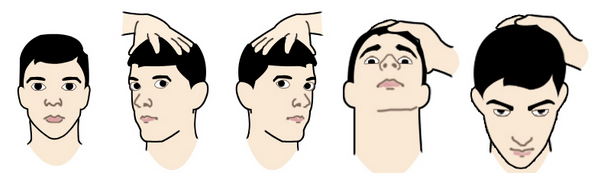
\includegraphics[scale=0.5]{images/vor.png}
  \footnote{\url{http://bit.ly/1Ox3Qd6}}
  This reflex functions to \textbf{stabilize images} on the retinas during \textbf{head movement} by producing \textbf{eye movements} in the direction opposite to head movement, thus preserving the image on the center of the visual field.
\end{frame}


\begin{frame}[fragile]
  \frametitle{Problem statement}
  \begin{quote}
    Computational models of the vestibulo-ocular reflex don't take into account the role of the nucleo-olivary inhibition
  \end{quote}
\end{frame}


\begin{frame}[fragile]
  \frametitle{Research question}
  \begin{quote}
    What's the role of the nucleo-olivary inhibition in the vestibulo-ocular reflex?
  \end{quote}
  \begin{block}{Fingerprints}
    \begin{itemize}
      \item NOI has a role in the eye-blink reflex
      \item There is extinction of the adaptive response in the absence of peripheral error
      \item VOR adaptation has a non-perfect performance, with a residual error proportional to the amount of cerebellar action required
    \end{itemize}
  \cite{Herreros2013b}
  \end{block}
\end{frame}


\begin{frame}[fragile]
  \frametitle{Hypothesis}
  \begin{quote}
    Adding nucleo-olivary inhibition on a detailed bottom-up state of the art vestibulo-ocular reflex computational model would offer a more
    parsimonious explanation of the experimental behavior of the reflex.
  \end{quote}
\end{frame}


% \begin{frame}[fragile]
%   \frametitle{Cerebellar cortex}
%   \begin{columns}[T]
%     \begin{column}[T]{5cm}
%       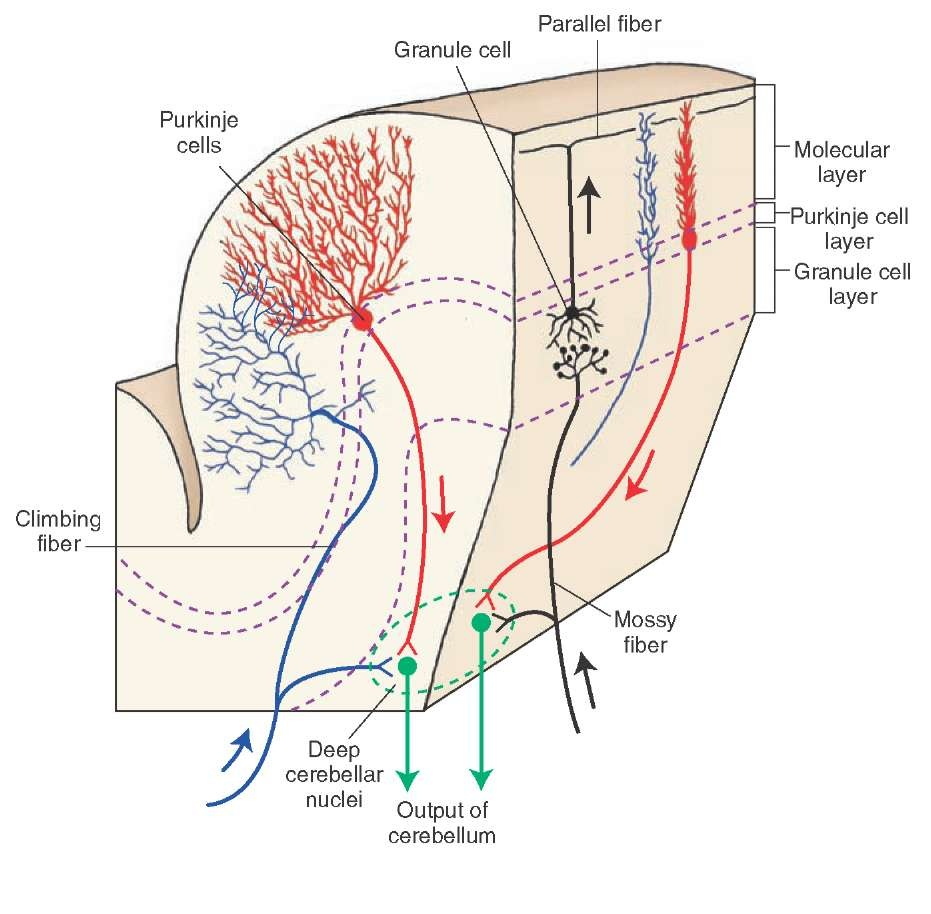
\includegraphics[scale=0.5]{images/tmp15F112.jpg}
%     \end{column}
%     \begin{column}[T]{5cm}
%       \begin{itemize}
%         \item Uniform structure throughout the cerebellum
%         \item Composed of repeated modules or microzones
%         \item Same cell types and connectivity
%         \item Functional units
%         \item Different inputs, different targets
%         \item Cerebellar algorithm
%       \end{itemize}
%     \end{column}
%   \end{columns}
%   \footnote{\url{http://bit.ly/1CioLvp}}
% \end{frame}


\section{State of the art}


\begin{frame}[fragile]
  \frametitle{Computational models of the VOR}
  \begin{itemize}
    \item Marr-Albus models
    \begin{itemize}
      \item Plasticity on the cerebellar cortex
      \item Climbing fibre as a teaching/error signal
      \item Quick adaptation
    \end{itemize}
    \item Plasticity on the brainstem
    \begin{itemize}
      \item Gain
      \item Long-term memory
      \item Slow adaptation
    \end{itemize}
    \item Multiple sites of plasticity
  \end{itemize}
\end{frame}


\section{Methods}


\begin{frame}[fragile]
  \frametitle{A detailed bottom-up model}
  This computational model is made bottom-up from physiological and behavioral observations.
  \begin{itemize}
    \item Plasticity on the cerebellar cortex
    \item Plasticity on the brainstem
    \item Delayed error signal
    \item White noise on the signals
    \item Contribution of interneurons
  \end{itemize}
  \cite{Clopath2014}
\end{frame}


\begin{frame}[fragile]
  \frametitle{Adding NOI to Clopath's model}
  \begin{columns}[T]
    \begin{column}[T]{5cm}
      Extinction on Clopath's model
      \begin{itemize}
        \item Weakly modulated by head movement (vestibular signal)
        \item Weights on cortical plasticity experiment a linear decay to their initial value
      \end{itemize}
    \end{column}
    \begin{column}[T]{5cm}
      Extinction on NOI model
      \begin{itemize}
        \item IO receives information from cortical afferents \cite{Najac2015}
        \item Extinction is defined as $k_noi*PC$
      \end{itemize}
    \end{column}
  \end{columns}
\end{frame}


\begin{frame}[fragile]
  \frametitle{VOR adaptation: Gain and phase}
\end{frame}


\begin{frame}[fragile]
  \frametitle{VOR phase reversal training protocol simulation}
  \begin{columns}[T]
    \begin{column}[T]{5cm}
      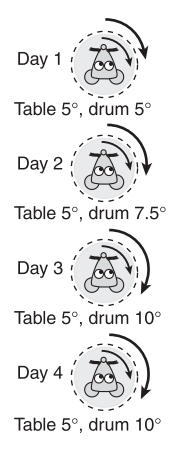
\includegraphics[scale=0.4]{images/vvor.png}
    \end{column}
    \begin{column}[T]{5cm}
      \begin{itemize}
        \item Day 1: VOR cancellation
        \item Day 2: VOR reversal with gain -0.5
        \item Day 3 and 4: Phase reversal with gain -1 (or gain 1 and phase $pi$)
      \end{itemize}
    \end{column}
  \end{columns}
\end{frame}


\begin{frame}[fragile]
  \frametitle{VOR with long extinction period simulation}
  \begin{columns}[T]
    \begin{column}[T]{5cm}
      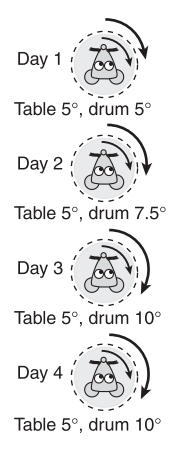
\includegraphics[scale=0.4]{images/vvor.png}
    \end{column}
    \begin{column}[T]{5cm}
      \begin{itemize}
        \item Day 1: VOR cancellation
        \item Day 2: VOR reversal with gain -0.5
        \item Day 3 and 4: Phase reversal with gain -1 (or gain 1 and phase $pi$)
        \item One week of light deprivation with vestibular stimulation
      \end{itemize}
    \end{column}
  \end{columns}
\end{frame}


\section{Results}


\begin{frame}[fragile]
  \frametitle{Reproducing Clopath's results}
  VOR adaptation
  \begin{columns}[onlytextwidth]
    \column{0.5\textwidth}
      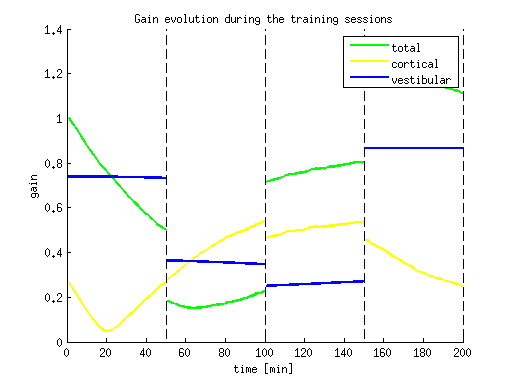
\includegraphics[scale=0.4]{../../simulations/parametric/html/clopath_27.png}
    \column{0.5\textwidth}
      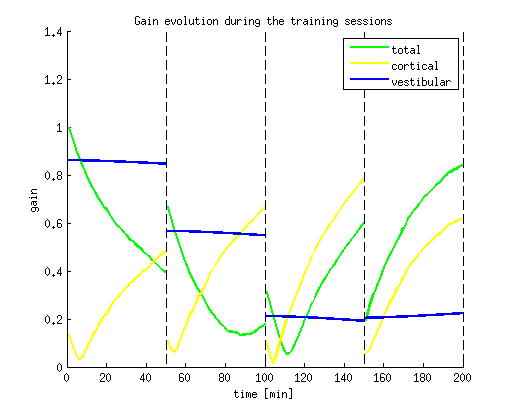
\includegraphics[scale=0.4]{../../simulations/parametric/html/noidifference_54.png}
  \end{columns}
\end{frame}


\begin{frame}[fragile]
  \frametitle{Extinction on Clopath's detailed model}
  After long periods of light deprivation, gain of the VOR reflex
  \begin{itemize}
    \item doesn't converge
    \item experiments a linear decay
  \end{itemize}
  \begin{columns}[onlytextwidth]
    \column{0.5\textwidth}
      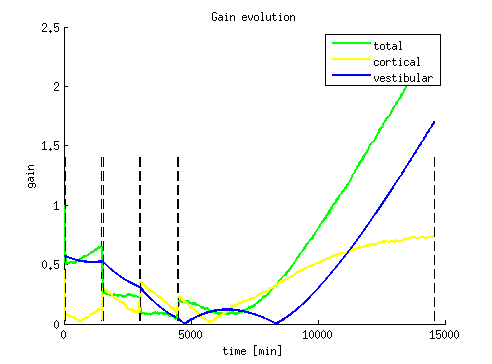
\includegraphics[scale=0.4]{../../simulations/parametric/html/longclopath_13.png}
    \column{0.5\textwidth}
      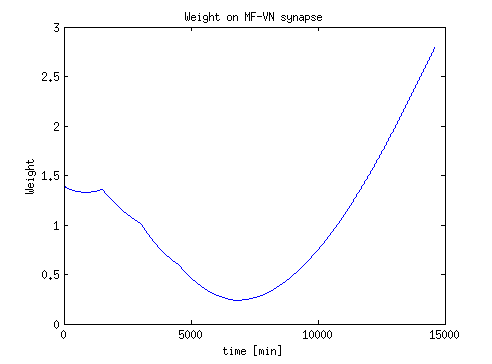
\includegraphics[scale=0.4]{../../simulations/parametric/html/longclopath_15.png}
  \end{columns}
\end{frame}


\begin{frame}[fragile]
  \frametitle{Extinction on Clopath's modified model with NOI}
  After long periods of light deprivation, gain of the VOR reflex
  \begin{itemize}
    \item converges to the initial state of the reflex
    \item experiments an exponential decay
  \end{itemize}
  \begin{columns}[onlytextwidth]
    \column{0.5\textwidth}
      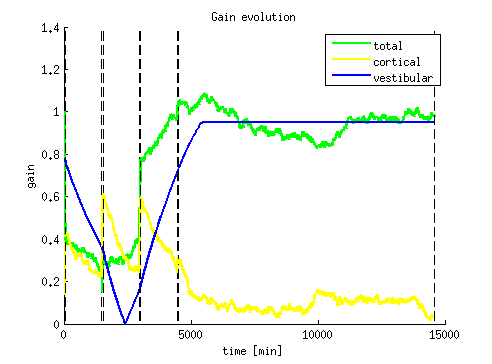
\includegraphics[scale=0.4]{../../simulations/parametric/html/longnoidifference_27.png}
    \column{0.5\textwidth}
      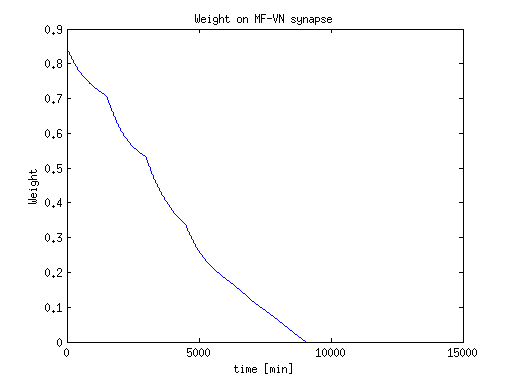
\includegraphics[scale=0.4]{../../simulations/parametric/html/longnoidifference_29.png}
  \end{columns}
\end{frame}


\begin{frame}[fragile]
  \frametitle{Cortical/nuclear memory balance}
  \begin{itemize}
    \item Cortical
      \begin{itemize}
        \item Quick adaptation
        \item Reacts on retinal slip error
        \item Short-term memory
      \end{itemize}
    \item Nuclear
      \begin{itemize}
        \item Slow adaptation
        \item Transference from cortical memory
        \item Long-term memory
      \end{itemize}
  \end{itemize}
\end{frame}


\section{Conclusions}


\begin{frame}[fragile]
  \frametitle{Conclusions}
  \begin{itemize}
    \item NOI explains extinction on VOR adaptation
    \item Extinction is triggered when vestibular information is available
    \item Teaching signal is modulated by cortical response (OCNO loop)
    \item Savings
    \item Limitations
    \begin{itemize}
      \item modulation on the PC
      \item there's always some nuclear transference
    \end{itemize}
  \end{itemize}
\end{frame}


\begin{frame}[fragile]
  \frametitle{Further work}
  More detailed bottom-up models
  \begin{itemize}
    \item transgenic mouse lines
    \item better electro-physiological recordings
    \item models with distributed plasticity
  \end{itemize}
\end{frame}


\section{References}


\begin{frame}[fragile]
  \frametitle{References}
  \bibliography{vornoi}
\end{frame}


\plain{Thank you}


\end{document}
